\section{DUNE Numerics Project}

\begin{frame}
	\frametitle{\secname}

	\begin{alertblock}{Distributed and Unified Numerics Environment (DUNE)}
		\note{
			Título: ``Una introducción a la caja de herramientas Dune en
			C++/Python para la solución de modelos matemáticos''.

			Se hará una breve presentación de la caja de herramientas
			modular Dune Numerics, biblioteca modular desarrollada en la
			Universidad de Heildeberg en C++ y Python, para resolver
			ecuaciones diferenciales parciales utilizando métodos basados
			en mallas, por ejemplo diferencias finitas, elementos finitos o
			volúmenes finitos.

			Es un software de código abierto bajo la licencia GNU General
			Public Licence 2, con binarios disponibles para las
			distribuciones Arch Linux en el repositorio arch4edu, Debian,
			openSUSE Tumbleweed y Ubuntu; también los scripts de
			compilación a través de Homebrew Formulae en macOS, los
			FreshPorts de FreeBSD y el Arch User Repository
			(AUR) en Arch Linux.

			Se mostrará la estructura general, algunos proyectos basados en
			Dune y algunas simulaciones de modelos matemáticos que incluyen
			este tipo de ecuaciones y sus respectivas soluciones, así como
			una implementación breve de Dune Numerics.
		}
		\begin{itemize}
			\item

			      Software de \alert{código abierto} bajo la licencia GNU
			      General Public Licence 2~\gpllicense{}.

			\item

			      Disponible en
			      \href{https://github.com/dune-copasi/homebrew-tap}{macOS},
			      \href{https://packages.debian.org/search?suite=sid&section=all&arch=any&searchon=sourcenames&keywords=dune-}{Debian}~\debian{},
			      \href{https://launchpad.net/~opm/+archive/ubuntu/ppa}{Ubuntu}~\ubuntu{},
			      \href{https://build.opensuse.org/search?search_text=dune-&search_for=2&name=1&attrib_type_id=}{openSUSE}~\opensuse{},
			      \href{https://aur.archlinux.org/packages/?O=0&SeB=n&K=dune-&outdated=&SB=n&SO=a&PP=50&do_Search=Ir}{\alert{Arch Linux}}~\archlinux{}
			      y \href{https://www.freshports.org/search.php?stype=name&method=match&query=dune-&num=20&orderby=category&orderbyupdown=asc&search=Search&format=html&branch=head}{FreeBSD}~\freebsd{}.

			\item

			      Conjunto de bibliotecas \alert{C++} con enlaces a
			      \href{https://pypi.org/search/?q=dune-}{\alert{Python}}.

			      \note{
				      Desarrollado con CMake, escrito en C++ con enlaces
				      Python a través de \texttt{pybind11}.

			      }

			\item

			      Utilizado en la resolución de
			      \alert{ecuaciones diferenciales parciales} e
			      implementación de métodos basados en mallas, por ejemplo
			      diferencias finitas, elementos finitos o volúmenes
			      finitos.
		\end{itemize}
	\end{alertblock}


	\begin{minipage}{0.45\textwidth}
		\begin{figure}[ht!]
			\centering
			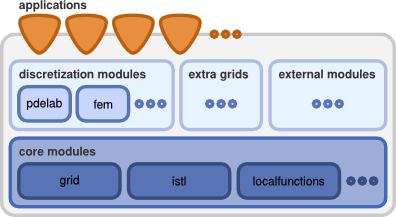
\includegraphics[height=3.2cm]{dunedesign}
			\caption*{\textbf{Origen:}~\url{dune-project.org/about/dune}.}
		\end{figure}
	\end{minipage}\qquad\qquad
	\begin{minipage}{0.45\textwidth}
		\begin{figure}[ht!]
			\centering
			\href{https://github.com/arch4edu/arch4edu}{
\includegraphics[height=2.8cm]{arch4edu}}\quad\quad
			\href{https://github.com/arch4edu/cactus}{
\includegraphics[height=2.8cm]{cactus}}
			\caption{Los binarios están disponible en el repositorio
				\alert{Arch Linux for Education}
				(Jingbei Li, Carlos Aznarán y otros, octubre 2022).
			}
		\end{figure}
	\end{minipage}
	\note{
		The easiest way to install the binaries are from Arch Linux Repository for Education.
		Jingbei Li, Carlos Aznarán, et al.
	}
\end{frame}

\begin{frame}
	\frametitle{\secname}
	\framesubtitle{\subsecname}

	\begin{columns}
		\begin{column}{0.5\textwidth}
			\begin{alertblock}{Proyectos que emplean DUNE}

				\

				\begin{itemize}
					\item

					      \url{https://dumux.org}

					      \

					\item

					      \url{https://opm-project.org}

					      \

					\item

					      \url{https://precice.org}

					      \

					\item

					      \url{https://www.zib.de/projects/kaskade7-finite-element-toolbox}
				\end{itemize}
			\end{alertblock}
		\end{column}

		\begin{column}{0.5\textwidth}
			\begin{figure}[ht!]
				\centering
				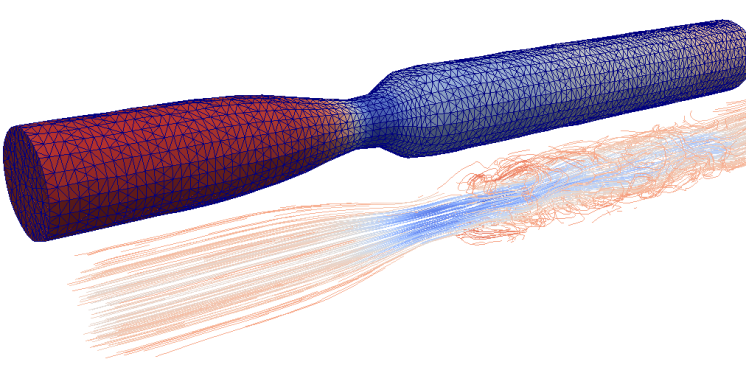
\includegraphics[width=7.5cm]{blood_girke}
				\caption*{\textbf{Origen:}~\url{dune-project.org/gallery}.}
			\end{figure}
		\end{column}
	\end{columns}
	\note{
		Presento las tres primeras páginas, la última versión estable de
		Dune es 2.8.0, pero la versión 2.9.0 se lanzó en octubre del 2022.

		DuMu\textsuperscript{x} es un simulador con modelos multifásicos
		de varias componentes, geomecánica, redes de poros,
		problemas de almacenamiento de gases, ley de Fick, Darcy,
		Richards, etc.

		El módulo opm-flow se puede apoyar del visualizador de simulación
		llamado \emph{Resinsight}.
	}
\end{frame}